\documentclass[12pt, a4paper]{article}
\usepackage[utf8]{inputenc}
\usepackage[T1]{fontenc}
\usepackage{beton}
\usepackage{eulervm}
\usepackage{amsmath}
\usepackage{bm}
\usepackage{microtype}
\usepackage{ellipsis}
\usepackage{booktabs}
\usepackage{graphicx}
\usepackage{color}
\usepackage{hyperref}
\usepackage{siunitx}
%
% \usepackage[medium, compact]{titlesec}
\DeclareFontSeriesDefault[rm]{bf}{sbc}
%%
%% Turing grid is 21 columns (of 1cm if we are using A4)
%% Usually 4 "big columns", each of 4 text cols plus 1 gutter col;
%% plus an additional gutter on the left.
\usepackage[top=2.82cm, bottom=2.82cm, left=3cm, textwidth=15cm, marginparsep=1cm, marginparwidth=2cm]{geometry}
%\usepackage[Ragged, size=footnote, shape=up]{sidenotesplus}
%% We used to use a two-column layout
% \setlength{\columnsep}{1cm}
\title{Legislation and Drones}
\author{James Geddes}
\date{\today}
%%
\newcommand{\eg}{\emph{e.g.}}
\newcommand{\ie}{\emph{i.e.}}
\newcommand{\isdef}{\mathrel{\stackrel{\text{def}}{=}}}
\hyphenation{anti-sym-met-ric}
%%
% \usepackage[backend=biber]{biblatex} 
%\addbibresource{BIBLIOGRAPHY-GOES-HERE.bib}
% \DefineBibliographyStrings{english}{
%   andothers = {\mkbibemph{et\addabbrvspace{al}\adddot}}
% }
%%
\begin{document}
\maketitle
\tableofcontents

\section{Legislation}

Roughly speaking, if government wants to change the world in some way,
it has three choices. It can subsidise---or buy---the thing that it wants;
it can impose a cost---a tax---on a thing that it doesn't want; or it can
explicitly tell people what to do and what not to do. This latter
approach is the regulatory solution.

In order to regulate, the government enacts \emph{primary
  legislation}, setting out the law. Sometimes the primary legislation
does not contain the full details of what the law is and these details
are later made law by \emph{secondary legislation}, usually by what is
called a ``statutory instrument.''

The government may then choose to devolve implementation of that
legislation to an arm's length body: a regulator. The regulator must
accept the law as given but has some freedom to tell others (typically
companies) what to do and what not to do. The regulator itself may
issue guidance on the legislation or describe how companies can
satisfy it, the regulator, that they have complied with the
legislation.

For further information, see the regulation section of the excellent
website \url{https://www.civilservant.org.uk/index.html}.

\begin{figure}[ht]
  \centering
  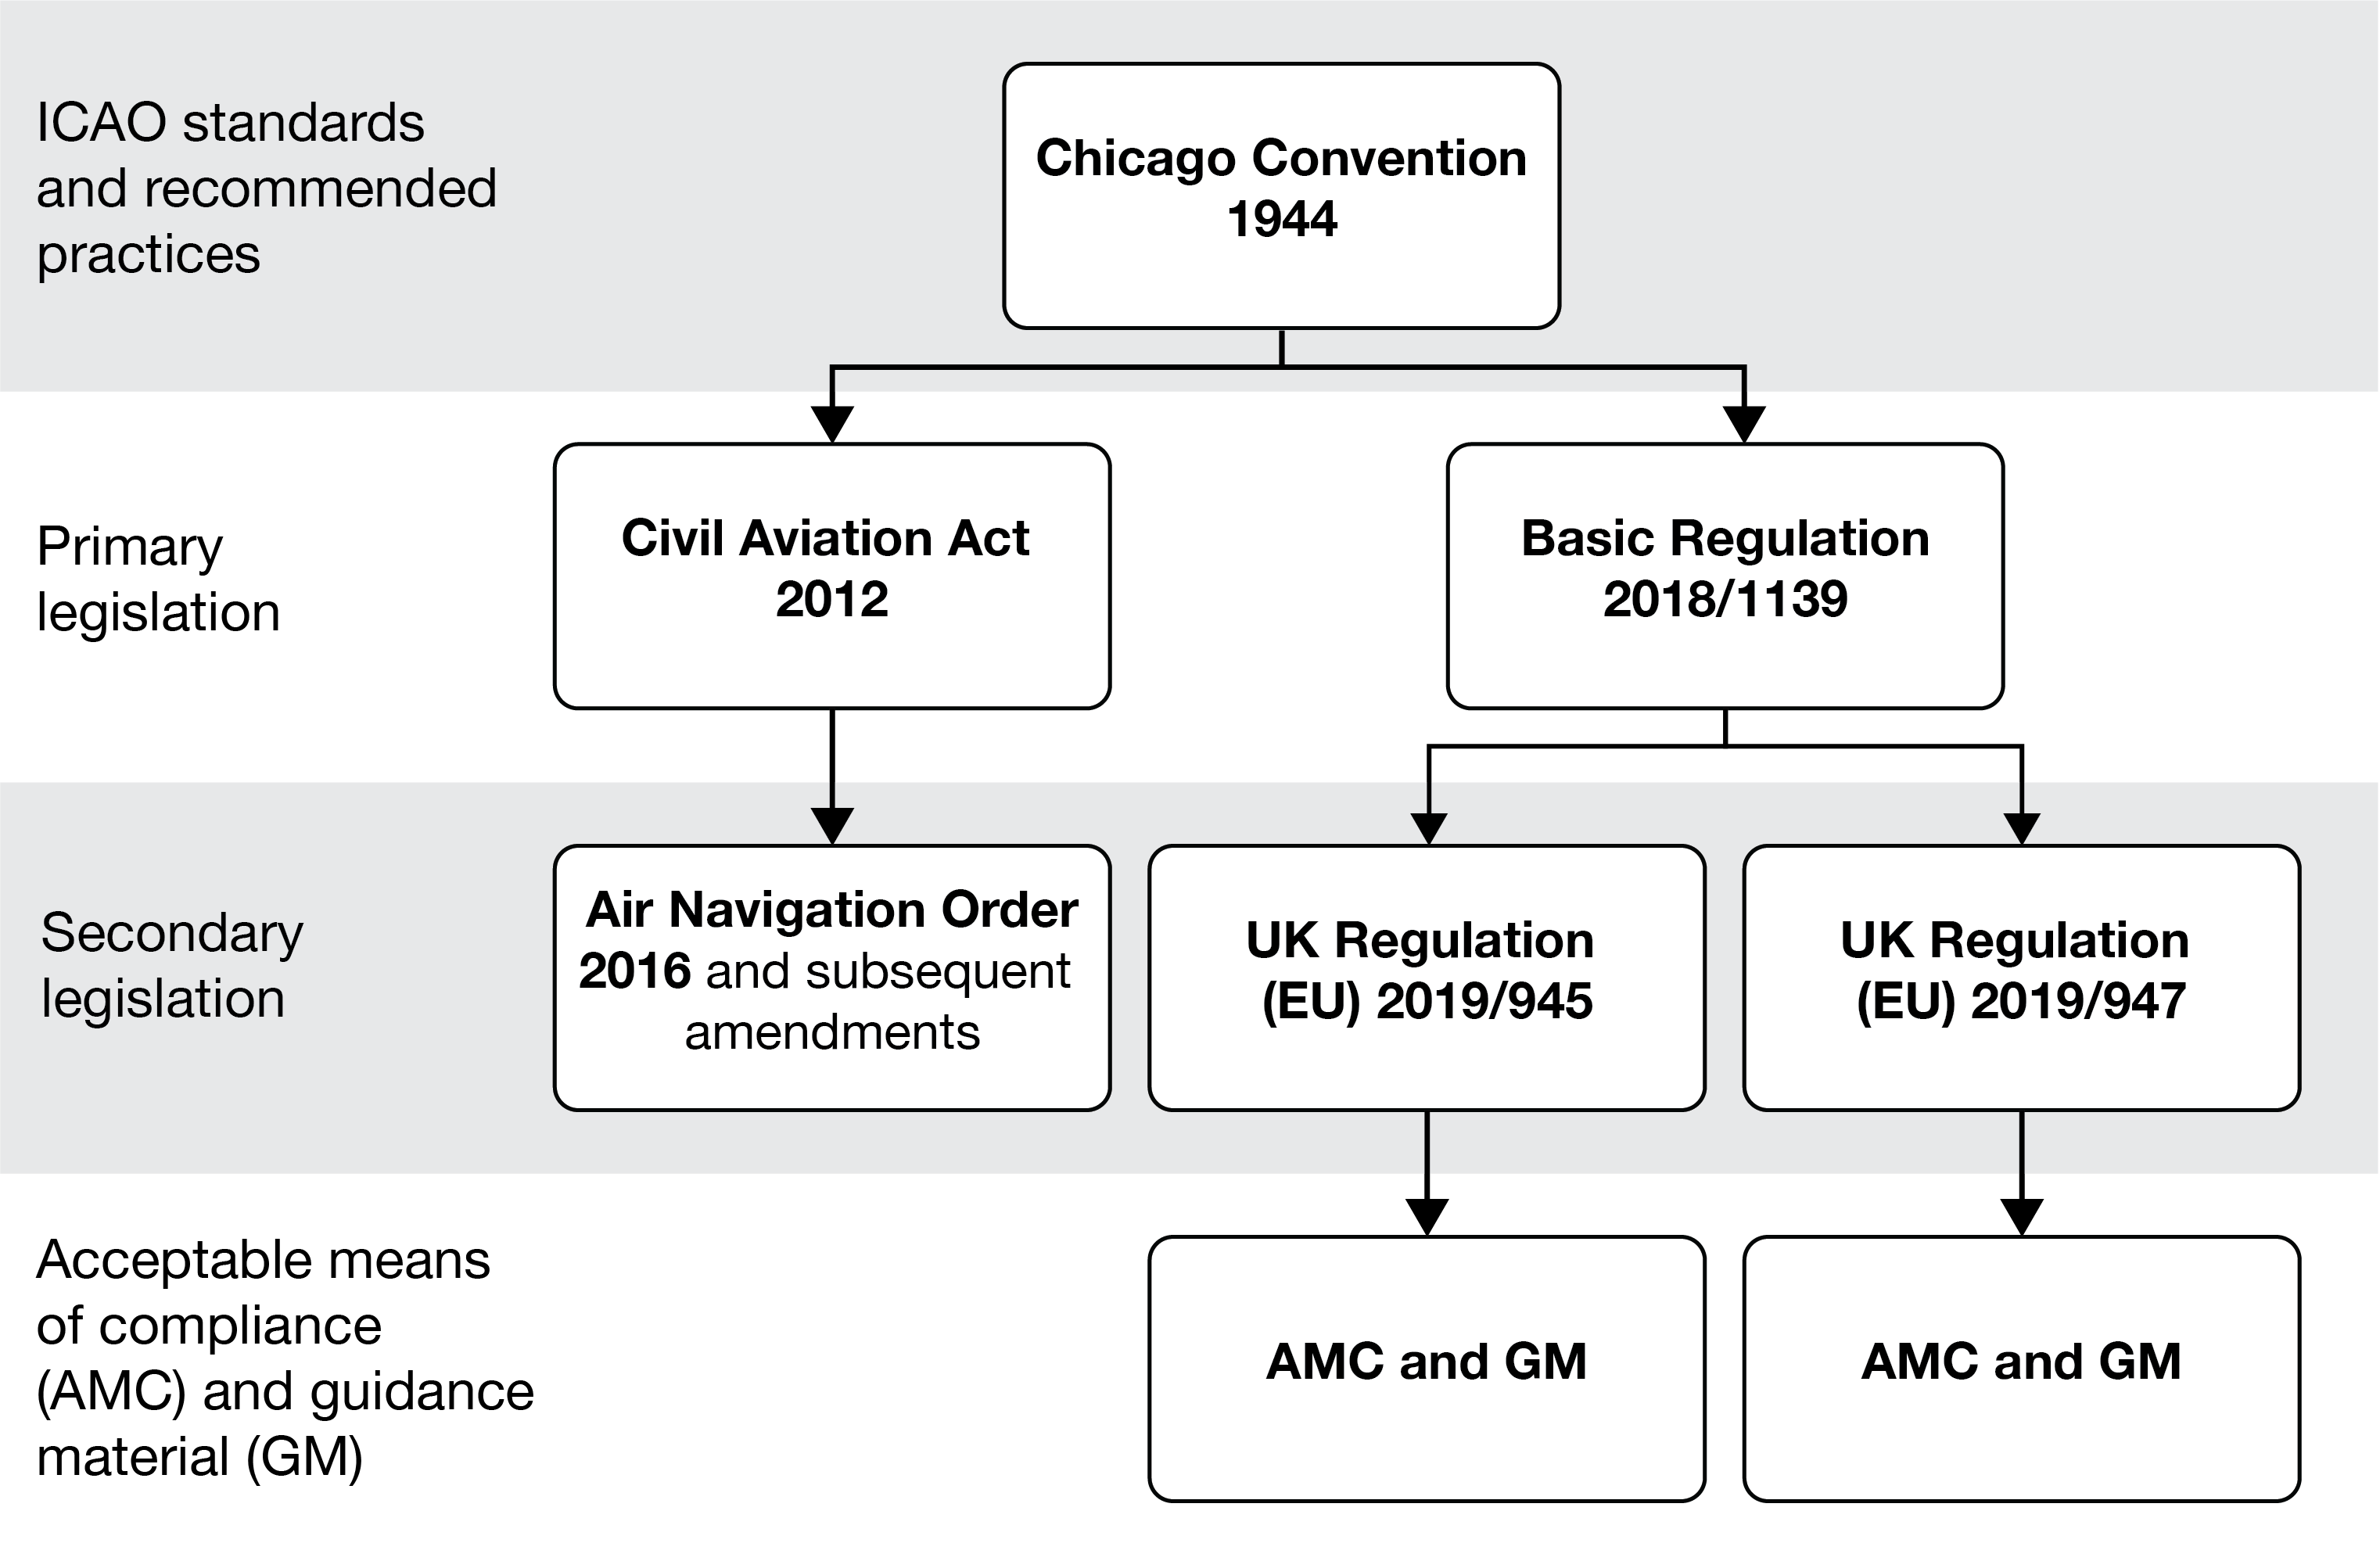
\includegraphics[width=0.8\textwidth]{figures/uk-uas-regulatory-framework.png}
  \caption{UK regulatory framwork for unmanned aircraft systems
    (drones). Source: CAA.\label{fig:drones}}
\end{figure}

\section{Drones}

Drones are unmanned flying machines, usually small, electrically
powered, and driven by downward-facing propellors (although fixed-wing
drones also exist). These days, the term seems to be ``UAS'' for
``Unmanned Aircraft System.''

The government department with overall responsibility for drones is
the Department for Transport (DfT) and the regulator is the Civil
Aviation Authority (CAA), although a manufacturer or operator might
also need to be aware of regulations around radio transmission (Ofcom)
and, indeed, privacy (the ICO).

The regulatory landscape for drones is shown in
figure~\ref{fig:drones}. The primary legislation that impacts drones
turns out to come from two sources:
\begin{enumerate}
\item The
  ``\href{https://www.legislation.gov.uk/eur/2018/1139/contents}{Basic
    Regulation}'' (Regulation (EU) 2018/1139) originally made by the
  EU and made UK law when the UK left the EU.\@ This legislation
  covers all aspects of aviation, not just drones: Unmanned aircraft
  are dealt with in Annex~IX.\@
\item The
  \href{https://www.legislation.gov.uk/ukpga/1982/16/contents}{Civil
    Aviation Act 2012}, which is the act of parliament that gives the
  CAA its authority.
\end{enumerate}

From the Basic Regulation follow two pieces of secondary legislatation
relevant to drones:
\begin{enumerate}
\item \href{https://www.legislation.gov.uk/eur/2019/947/contents}{The
    UAS Implementing Regulation} (UK Regulation (EU) 2019/947), which
  ``lays down detailed provisions for the operation of unmanned
  aircraft systems as well as for personnel, including remote pilots
  and organisations involved in those operations''; and
\item
  \href{https://www.legislation.gov.uk/eur/2019/945/contents}{The UAS
    Delegated Regulations} (Commission
    Delegated Regulation (EU) 2019/945), which ``lays down the requirements for the design and
  manufacture of unmanned aircraft systems (‘UAS’) intended to be
  operated under the rules and conditions defined in Implementing
  Regulation (EU) 2019/947 [...]''
\end{enumerate}

From the Civil Aviation Act there follows one piece of secondary
legislation relevant to drones:
\begin{enumerate}
\item \href{https://www.legislation.gov.uk/uksi/2016/765/contents}{The
    Air Navigation Order 2016/765} and subsequent amendments,
  especially the
  \href{https://www.legislation.gov.uk/uksi/2020/1555/contents/made}{The
    Air Navigation (Amendment) Order 2020} (also known as SI
  2020/1555) which made amendments relevant to UAS.\@
\end{enumerate}

Finally, the CAA itself issues guidance:
\begin{enumerate}
\item on the Air Navigation (Amendment) Order (as
  \href{https://www.caa.co.uk/our-work/publications/documents/content/cap2013/}{CAP
    2013}); and
\item for the UAS Implementing Regulation (as ``Acceptable Means of Compliance'' and ``Guidance
  Material,'' \href{https://regulatorylibrary.caa.co.uk/2019-947/Content/UAS947_1.htm}{AMC
    and GM}).
\end{enumerate}

This guidance clarifies the meaning of parts of the legislation: by
saying what certain terms mean to the regulator. For example, that
``autonomous operation'' does not mean ``automatic operation;'' that
``Visual Line of Sight operation'' means that certain features must be
distinguishable by the naked eye---it's not enough to be able to just
make out the drone in the distance; and so on.

The CAA also publishes a \href{https://www.caa.co.uk/drones/}{web
  page} of additional explanatory and informational material to help
drone operators comply with the law (as the CAA sees it) as well as
the ``\href{https://register-drones.caa.co.uk/drone-code}{Drone and
  Model Aircraft Code}.'' These instructions bring together the
regulations in a more straightforward way for someone who just wants
to fly a drone.

\appendix
\section{i.AI and Lex}

i.AI is working in the same area. One of their projects is
``\href{https://ai.gov.uk/projects/parlex-and-lex/}{Lex},'' a tool
that is designed to support searches of UK legislation. It seems to be
essentially RAG (which is of course very sensible). There is some
additional work apparently being done on building a
\href{https://ai.gov.uk/blogs/understanding-legislative-networks-building-a-knowledge-graph-of-uk-legislation/}{``knowledge
  graph'' of legislation} (and
\href{https://ai.gov.uk/blogs/understanding-legislative-networks-building-a-knowledge-graph-of-uk-legislation/}{GitHub
  repo}).

\end{document}
